\documentclass[]{article}
\usepackage{lmodern}
\usepackage{amssymb,amsmath}
\usepackage{ifxetex,ifluatex}
\usepackage{fixltx2e} % provides \textsubscript
\ifnum 0\ifxetex 1\fi\ifluatex 1\fi=0 % if pdftex
  \usepackage[T1]{fontenc}
  \usepackage[utf8]{inputenc}
\else % if luatex or xelatex
  \ifxetex
    \usepackage{mathspec}
  \else
    \usepackage{fontspec}
  \fi
  \defaultfontfeatures{Ligatures=TeX,Scale=MatchLowercase}
\fi
% use upquote if available, for straight quotes in verbatim environments
\IfFileExists{upquote.sty}{\usepackage{upquote}}{}
% use microtype if available
\IfFileExists{microtype.sty}{%
\usepackage{microtype}
\UseMicrotypeSet[protrusion]{basicmath} % disable protrusion for tt fonts
}{}
\usepackage[margin=1in]{geometry}
\usepackage{hyperref}
\hypersetup{unicode=true,
            pdfborder={0 0 0},
            breaklinks=true}
\urlstyle{same}  % don't use monospace font for urls
\usepackage{color}
\usepackage{fancyvrb}
\newcommand{\VerbBar}{|}
\newcommand{\VERB}{\Verb[commandchars=\\\{\}]}
\DefineVerbatimEnvironment{Highlighting}{Verbatim}{commandchars=\\\{\}}
% Add ',fontsize=\small' for more characters per line
\usepackage{framed}
\definecolor{shadecolor}{RGB}{248,248,248}
\newenvironment{Shaded}{\begin{snugshade}}{\end{snugshade}}
\newcommand{\KeywordTok}[1]{\textcolor[rgb]{0.13,0.29,0.53}{\textbf{#1}}}
\newcommand{\DataTypeTok}[1]{\textcolor[rgb]{0.13,0.29,0.53}{#1}}
\newcommand{\DecValTok}[1]{\textcolor[rgb]{0.00,0.00,0.81}{#1}}
\newcommand{\BaseNTok}[1]{\textcolor[rgb]{0.00,0.00,0.81}{#1}}
\newcommand{\FloatTok}[1]{\textcolor[rgb]{0.00,0.00,0.81}{#1}}
\newcommand{\ConstantTok}[1]{\textcolor[rgb]{0.00,0.00,0.00}{#1}}
\newcommand{\CharTok}[1]{\textcolor[rgb]{0.31,0.60,0.02}{#1}}
\newcommand{\SpecialCharTok}[1]{\textcolor[rgb]{0.00,0.00,0.00}{#1}}
\newcommand{\StringTok}[1]{\textcolor[rgb]{0.31,0.60,0.02}{#1}}
\newcommand{\VerbatimStringTok}[1]{\textcolor[rgb]{0.31,0.60,0.02}{#1}}
\newcommand{\SpecialStringTok}[1]{\textcolor[rgb]{0.31,0.60,0.02}{#1}}
\newcommand{\ImportTok}[1]{#1}
\newcommand{\CommentTok}[1]{\textcolor[rgb]{0.56,0.35,0.01}{\textit{#1}}}
\newcommand{\DocumentationTok}[1]{\textcolor[rgb]{0.56,0.35,0.01}{\textbf{\textit{#1}}}}
\newcommand{\AnnotationTok}[1]{\textcolor[rgb]{0.56,0.35,0.01}{\textbf{\textit{#1}}}}
\newcommand{\CommentVarTok}[1]{\textcolor[rgb]{0.56,0.35,0.01}{\textbf{\textit{#1}}}}
\newcommand{\OtherTok}[1]{\textcolor[rgb]{0.56,0.35,0.01}{#1}}
\newcommand{\FunctionTok}[1]{\textcolor[rgb]{0.00,0.00,0.00}{#1}}
\newcommand{\VariableTok}[1]{\textcolor[rgb]{0.00,0.00,0.00}{#1}}
\newcommand{\ControlFlowTok}[1]{\textcolor[rgb]{0.13,0.29,0.53}{\textbf{#1}}}
\newcommand{\OperatorTok}[1]{\textcolor[rgb]{0.81,0.36,0.00}{\textbf{#1}}}
\newcommand{\BuiltInTok}[1]{#1}
\newcommand{\ExtensionTok}[1]{#1}
\newcommand{\PreprocessorTok}[1]{\textcolor[rgb]{0.56,0.35,0.01}{\textit{#1}}}
\newcommand{\AttributeTok}[1]{\textcolor[rgb]{0.77,0.63,0.00}{#1}}
\newcommand{\RegionMarkerTok}[1]{#1}
\newcommand{\InformationTok}[1]{\textcolor[rgb]{0.56,0.35,0.01}{\textbf{\textit{#1}}}}
\newcommand{\WarningTok}[1]{\textcolor[rgb]{0.56,0.35,0.01}{\textbf{\textit{#1}}}}
\newcommand{\AlertTok}[1]{\textcolor[rgb]{0.94,0.16,0.16}{#1}}
\newcommand{\ErrorTok}[1]{\textcolor[rgb]{0.64,0.00,0.00}{\textbf{#1}}}
\newcommand{\NormalTok}[1]{#1}
\usepackage{longtable,booktabs}
\usepackage{graphicx,grffile}
\makeatletter
\def\maxwidth{\ifdim\Gin@nat@width>\linewidth\linewidth\else\Gin@nat@width\fi}
\def\maxheight{\ifdim\Gin@nat@height>\textheight\textheight\else\Gin@nat@height\fi}
\makeatother
% Scale images if necessary, so that they will not overflow the page
% margins by default, and it is still possible to overwrite the defaults
% using explicit options in \includegraphics[width, height, ...]{}
\setkeys{Gin}{width=\maxwidth,height=\maxheight,keepaspectratio}
\IfFileExists{parskip.sty}{%
\usepackage{parskip}
}{% else
\setlength{\parindent}{0pt}
\setlength{\parskip}{6pt plus 2pt minus 1pt}
}
\setlength{\emergencystretch}{3em}  % prevent overfull lines
\providecommand{\tightlist}{%
  \setlength{\itemsep}{0pt}\setlength{\parskip}{0pt}}
\setcounter{secnumdepth}{0}
% Redefines (sub)paragraphs to behave more like sections
\ifx\paragraph\undefined\else
\let\oldparagraph\paragraph
\renewcommand{\paragraph}[1]{\oldparagraph{#1}\mbox{}}
\fi
\ifx\subparagraph\undefined\else
\let\oldsubparagraph\subparagraph
\renewcommand{\subparagraph}[1]{\oldsubparagraph{#1}\mbox{}}
\fi

%%% Use protect on footnotes to avoid problems with footnotes in titles
\let\rmarkdownfootnote\footnote%
\def\footnote{\protect\rmarkdownfootnote}

%%% Change title format to be more compact
\usepackage{titling}

% Create subtitle command for use in maketitle
\newcommand{\subtitle}[1]{
  \posttitle{
    \begin{center}\large#1\end{center}
    }
}

\setlength{\droptitle}{-2em}

  \title{}
    \pretitle{\vspace{\droptitle}}
  \posttitle{}
    \author{}
    \preauthor{}\postauthor{}
    \date{}
    \predate{}\postdate{}
  
% header for lbg_hs2017_w13_exmsol.Rmd
\usepackage{amsmath}

\newcommand{\points}[1]
{\begin{flushright}\textbf{#1}\end{flushright}}
\newcommand{\sol}
{\vspace{2ex}\textbf{Solution}:}

\begin{document}

\thispagestyle{empty}

\begin{tabular}{l}
ETH Zurich \\
D-USYS\\
Institute of Agricultural Sciences\\
\end{tabular}

\vspace{15ex}

\begin{center}
\huge
Exam Solutions \\ \vspace{1ex}
Livestock Breeding and Genomics \\  \vspace{1ex}
FS 2017 \\

\normalsize
\vspace{7ex}
Peter von Rohr 
\end{center}

\vspace{7ex}

\begin{tabular}{p{5cm}lr}
  & \textsc{Date}  & \textsc{\emph{22. December 2017}} \\
  & \textsc{Begin} & \textsc{\emph{09:15 }}\\
  & \textsc{End}   & \textsc{\emph{11:15 }}\\ 
\end{tabular}

\vspace{5ex} \large

\begin{tabular}{p{2.5cm}p{3cm}p{6cm}}
  &  Name:     &  \\
  &            &  \\
  &  Legi-Nr:  & \\
\end{tabular}

\normalsize

\vspace{9ex}

\begin{center}
\begin{tabular}{|p{3cm}|c|c|}
\hline
Problem  &  Maximal Number of Points  &  Number of Points Reached \\
\hline
1        &  48         & \\
\hline
2        &  22         & \\
\hline
3        &  30         & \\
\hline
4        &  30          & \\
\hline
5        &  29          & \\
\hline
Total    &  159    & \\
\hline
\end{tabular}
\end{center}

\clearpage
\pagebreak

\subsection{Problem 1 Relationship and
Inbreeding}\label{problem-1-relationship-and-inbreeding}

We are given the following pedigree

\begin{verbatim}
##   sire  dam
## 1 <NA> <NA>
## 2 <NA> <NA>
## 3    1    2
## 4    1    3
## 5    4    2
## 6    4    5
\end{verbatim}

\begin{enumerate}
\item[a)] Use the given pedigree to construct the numerator relationship matrix $A$
\points{36}
\end{enumerate}

\sol

\begin{Shaded}
\begin{Highlighting}[]
\NormalTok{(matA <-}\StringTok{ }\KeywordTok{as.matrix}\NormalTok{(}\KeywordTok{getA}\NormalTok{(}\DataTypeTok{ped =}\NormalTok{ ped)))}
\end{Highlighting}
\end{Shaded}

\begin{verbatim}
##        1      2      3    4      5      6
## 1 1.0000 0.0000 0.5000 0.75 0.3750 0.5625
## 2 0.0000 1.0000 0.5000 0.25 0.6250 0.4375
## 3 0.5000 0.5000 1.0000 0.75 0.6250 0.6875
## 4 0.7500 0.2500 0.7500 1.25 0.7500 1.0000
## 5 0.3750 0.6250 0.6250 0.75 1.1250 0.9375
## 6 0.5625 0.4375 0.6875 1.00 0.9375 1.3750
\end{verbatim}

\clearpage
\pagebreak

\begin{enumerate}
\item[b)] Which elements of the matrix $A$ contain the inbreeding coefficient $F_5$ of animal $5$? What is the value of the inbreeding coefficient $F_5$?
\points{8}
\end{enumerate}

\sol

The following elements contain \(F_5\) \[(2,4), (4,2), (5,5)\]

The value of \(F_5\) corresponds to

\[F_5 = 0.125\]

\clearpage
\pagebreak

\begin{enumerate}
\item[c)] Which parents would $5$ need to have, such that $F_5 = 0$ would hold?
\points{4}
\end{enumerate}

\sol

Because only \(1\) and \(2\) are not related, these would be the only
parents with which \(F_5 = 0\) would be true.

\clearpage
\pagebreak

\subsection{Problem 2 Variance Components
Estimation}\label{problem-2-variance-components-estimation}

We are given the following dataset for the traits body weight and breast
circumference for cattle.

\begin{longtable}[]{@{}rlrr@{}}
\toprule
Animal & Herd & BodyWeight & BreastCircumference\tabularnewline
\midrule
\endhead
1 & 2 & 669 & 161\tabularnewline
2 & 1 & 635 & 144\tabularnewline
3 & 1 & 631 & 151\tabularnewline
4 & 1 & 632 & 155\tabularnewline
5 & 1 & 642 & 167\tabularnewline
6 & 2 & 676 & 165\tabularnewline
7 & 1 & 645 & 163\tabularnewline
8 & 2 & 686 & 171\tabularnewline
9 & 1 & 633 & 138\tabularnewline
10 & 1 & 641 & 170\tabularnewline
\bottomrule
\end{longtable}

\begin{enumerate}
\item[a)] What is the value for the estimated resiudal variance for the trait `body weight`, when the following assumptions are met.
\points{12}
\end{enumerate}

In a first model, we assume that \texttt{body\ weight} is influenced by
the herd leading to the following model

\[y = Xb + e\]

\begin{tabular}{lll}
wobei  &  & \\
       &  $y$  &  vector of observations for `body weight` \\
       &  $b$  &  vector of herd effects \\
       &  $X$  &  incidence matrix linking observations to herd effects \\
       &  $e$  &  vector with random resiudals with $E[e] = 0$ and $var(e) = I \sigma^2$
\end{tabular}

The estimates of the herd effects were computed using the function
\texttt{lm()} in R. The statement for that is given below

\begin{Shaded}
\begin{Highlighting}[]
\NormalTok{lm_gewicht <-}\StringTok{ }\KeywordTok{lm}\NormalTok{(BodyWeight }\OperatorTok{~}\StringTok{ }\OperatorTok{-}\DecValTok{1} \OperatorTok{+}\StringTok{ }\NormalTok{Herd, }\DataTypeTok{data =}\NormalTok{ dfWtBc)}
\KeywordTok{round}\NormalTok{(}\KeywordTok{coefficients}\NormalTok{(lm_gewicht), }\DataTypeTok{digits =} \DecValTok{1}\NormalTok{)}
\end{Highlighting}
\end{Shaded}

\begin{verbatim}
## Herd1 Herd2 
##   637   677
\end{verbatim}

\subsubsection{Your task}\label{your-task}

Estimate the residual variance \(\sigma^2\) for the given model for
\texttt{body\ weight} with the method based on the residuals. The same
value for the residual variance could also be obtained from the Output
of the \texttt{summary()}-function in R.

\sol

The vector of residuals \(e\) is

\begin{Shaded}
\begin{Highlighting}[]
\NormalTok{(vec_residuals <-}\StringTok{ }\KeywordTok{residuals}\NormalTok{(lm_gewicht))}
\end{Highlighting}
\end{Shaded}

\begin{verbatim}
##  1  2  3  4  5  6  7  8  9 10 
## -8 -2 -6 -5  5 -1  8  9 -4  4
\end{verbatim}

The estimated residual variance corresponds to the squared residuals
divided by the degrees of freedom \(df_e = n - p\) where \(n\)
corresponds to the number of observations and \(p\) corresponds to the
number of herd effects. Therefore \(df_e = 10 - 2 = 8\).

The estimated residual variance and the residual standard deviation are

\begin{Shaded}
\begin{Highlighting}[]
\NormalTok{(ssq_res <-}\StringTok{ }\KeywordTok{crossprod}\NormalTok{(vec_residuals))}
\end{Highlighting}
\end{Shaded}

\begin{verbatim}
##      [,1]
## [1,]  332
\end{verbatim}

\begin{Shaded}
\begin{Highlighting}[]
\NormalTok{(n_sigma2_hat <-}\StringTok{ }\NormalTok{ssq_res}\OperatorTok{/}\NormalTok{(n_nr_obs }\OperatorTok{-}\StringTok{ }\KeywordTok{length}\NormalTok{(}\KeywordTok{coefficients}\NormalTok{(lm_gewicht))))}
\end{Highlighting}
\end{Shaded}

\begin{verbatim}
##      [,1]
## [1,] 41.5
\end{verbatim}

\begin{Shaded}
\begin{Highlighting}[]
\NormalTok{(n_sigma_hat <-}\StringTok{ }\KeywordTok{sqrt}\NormalTok{(n_sigma2_hat))}
\end{Highlighting}
\end{Shaded}

\begin{verbatim}
##          [,1]
## [1,] 6.442049
\end{verbatim}

As a check, we compare the result to the output of R

\begin{Shaded}
\begin{Highlighting}[]
\KeywordTok{summary}\NormalTok{(lm_gewicht)}
\end{Highlighting}
\end{Shaded}

\begin{verbatim}
## 
## Call:
## lm(formula = BodyWeight ~ -1 + Herd, data = dfWtBc)
## 
## Residuals:
##    Min     1Q Median     3Q    Max 
##  -8.00  -4.75  -1.50   4.75   9.00 
## 
## Coefficients:
##       Estimate Std. Error t value Pr(>|t|)    
## Herd1  637.000      2.435   261.6  < 2e-16 ***
## Herd2  677.000      3.719   182.0 9.29e-16 ***
## ---
## Signif. codes:  0 '***' 0.001 '**' 0.01 '*' 0.05 '.' 0.1 ' ' 1
## 
## Residual standard error: 6.442 on 8 degrees of freedom
## Multiple R-squared:  0.9999, Adjusted R-squared:  0.9999 
## F-statistic: 5.079e+04 on 2 and 8 DF,  p-value: < 2.2e-16
\end{verbatim}

\clearpage
\pagebreak

\begin{enumerate}
\item[b)] What is the difference between the estimated residual variance from Problem 2a) and the estimate of the residual variance based on Maximum Likelhood? 
\points{6}
\end{enumerate}

\subsubsection{Your Task}\label{your-task-1}

\begin{itemize}
\tightlist
\item
  Describe the difference between the two estimates
\item
  Compute the value of the Maximum-Likelhood-Estimate for the residual
  variance
\item
  Which of the two estimate is considered to be ``better'' than the
  other?
\end{itemize}

\sol

\begin{itemize}
\tightlist
\item
  With the Maximum-Likelihood estimate the degrees of freedom \(p\) for
  the estimation of the fixed effects are not considered
\item
  The value of the estimated residual variance is the same as in a), but
  the factor with which the sums of squares are multiplied is \(1/n\)
  and not \(1/(n-p)\). Hence, we get \[\widehat{\sigma^2_{ML}} = 33.2\]
\item
  The estimate computed in a) based on the residuals is unbiased and is
  considered better.
\end{itemize}

\clearpage
\pagebreak

\begin{enumerate}
\item[c)] When the body weight of animal $11$ in herd $1$ was recorded, the scale broke down.  The body weight of animal $11$ is estimated such that it is within the range of $\pm 2$ standard deviations around the mean body weight for herd $1$. 
\points{4}
\end{enumerate}

\subsubsection{Hints}\label{hints}

\begin{itemize}
\tightlist
\item
  Use the estimate of the standard deviation computed from Problem 2a)
\item
  If you could not solve Problem 2a), use a value of \(10\) as an
  approximation of the estimated residuals standard deviation.
\end{itemize}

\sol

\begin{Shaded}
\begin{Highlighting}[]
\NormalTok{(n_av_gew_btr1 <-}\StringTok{ }\KeywordTok{mean}\NormalTok{(dfWtBc}\OperatorTok{$}\NormalTok{Gewicht[dfWtBc}\OperatorTok{$}\NormalTok{Betrieb }\OperatorTok{==}\StringTok{ }\DecValTok{1}\NormalTok{]))}
\end{Highlighting}
\end{Shaded}

\begin{verbatim}
## Warning in mean.default(dfWtBc$Gewicht[dfWtBc$Betrieb == 1]): argument is
## not numeric or logical: returning NA
\end{verbatim}

\begin{verbatim}
## [1] NA
\end{verbatim}

\begin{Shaded}
\begin{Highlighting}[]
\NormalTok{(n_lower <-}\StringTok{  }\NormalTok{n_av_gew_btr1 }\OperatorTok{-}\StringTok{ }\DecValTok{2}\OperatorTok{*}\StringTok{ }\NormalTok{n_sigma_hat)}
\end{Highlighting}
\end{Shaded}

\begin{verbatim}
##      [,1]
## [1,]   NA
\end{verbatim}

\begin{Shaded}
\begin{Highlighting}[]
\NormalTok{(n_upper <-}\StringTok{ }\NormalTok{n_av_gew_btr1 }\OperatorTok{+}\StringTok{ }\DecValTok{2}\OperatorTok{*}\StringTok{ }\NormalTok{n_sigma_hat)}
\end{Highlighting}
\end{Shaded}

\begin{verbatim}
##      [,1]
## [1,]   NA
\end{verbatim}

\clearpage
\pagebreak

\subsection{Problem 3 Livestock
Breeding}\label{problem-3-livestock-breeding}

\begin{enumerate}
\item[a)] What is the difference between livestock population and wildlife populations with respect to the terms `selection` and `mating`? Please complete the following table.
\points{8}
\end{enumerate}

\vspace{3ex}

\begin{center}
\begin{tabular}{p{2cm}|p{5.5cm}|p{5.5cm}}
\hline
& & \\
Population & Selection & Mating \\
& & \\
\hline
& & \\
& & \\
Wildlife &  &  \\ 
& & \\
& & \\
\hline
& & \\
& & \\
Livestock &  &  \\ 
& & \\
& & \\
\hline
\end{tabular}
\end{center}

\vspace{5ex} \sol

\vspace{3ex}

\begin{longtable}[]{@{}lll@{}}
\toprule
Population & Selektion & Anpaarung\tabularnewline
\midrule
\endhead
Wildlife & Natural selection based on environment & random
mating\tabularnewline
Lifestock & artificial and directed selection & planned
mating\tabularnewline
\bottomrule
\end{longtable}

\clearpage
\pagebreak

\begin{enumerate}
\item[b)] In a selection scheme based on phenotypic observations, the distribution of the parents and the progeny is compared in the following diagram. Please put names on the labels in the following diagram.
\points{12}
\end{enumerate}

\begin{center}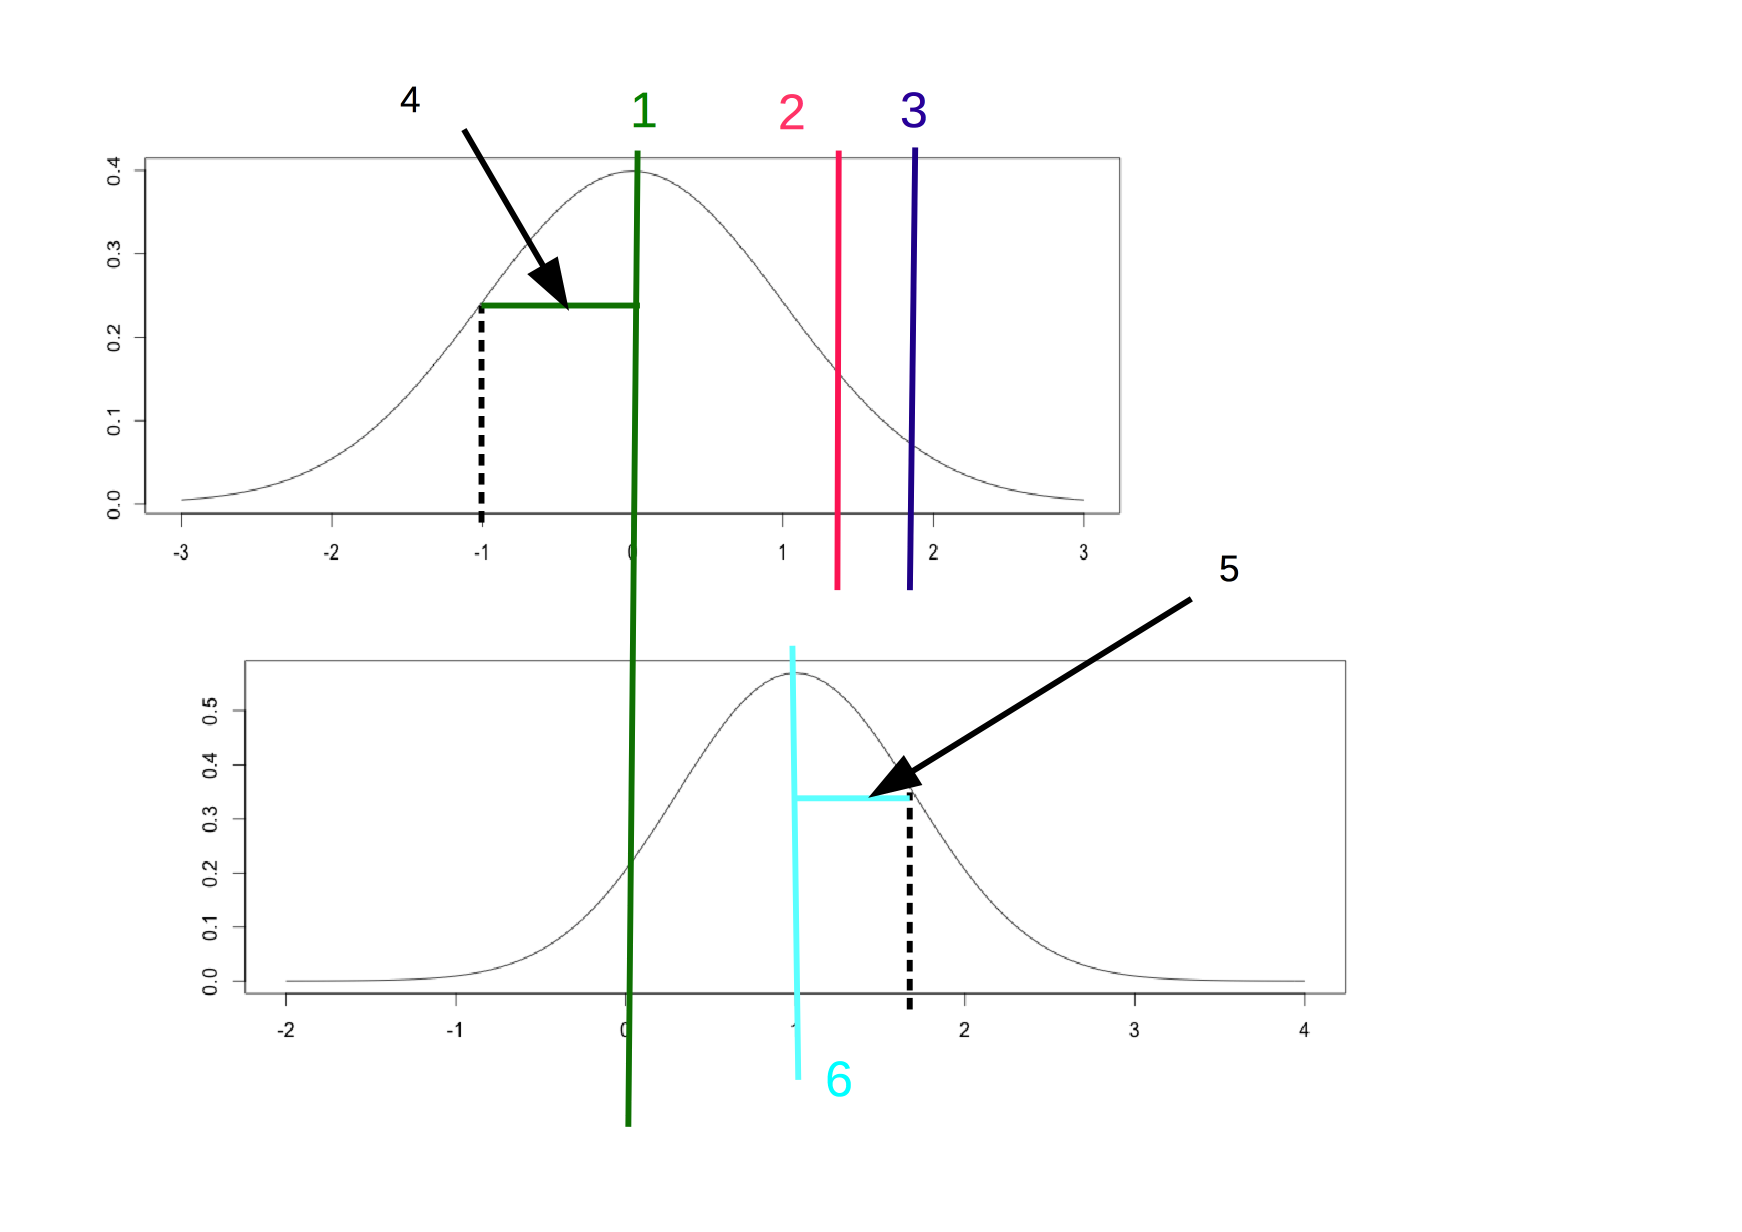
\includegraphics{png/GerichteteSelektionElternNk} \end{center}

\clearpage
\pagebreak

\sol

\begin{center}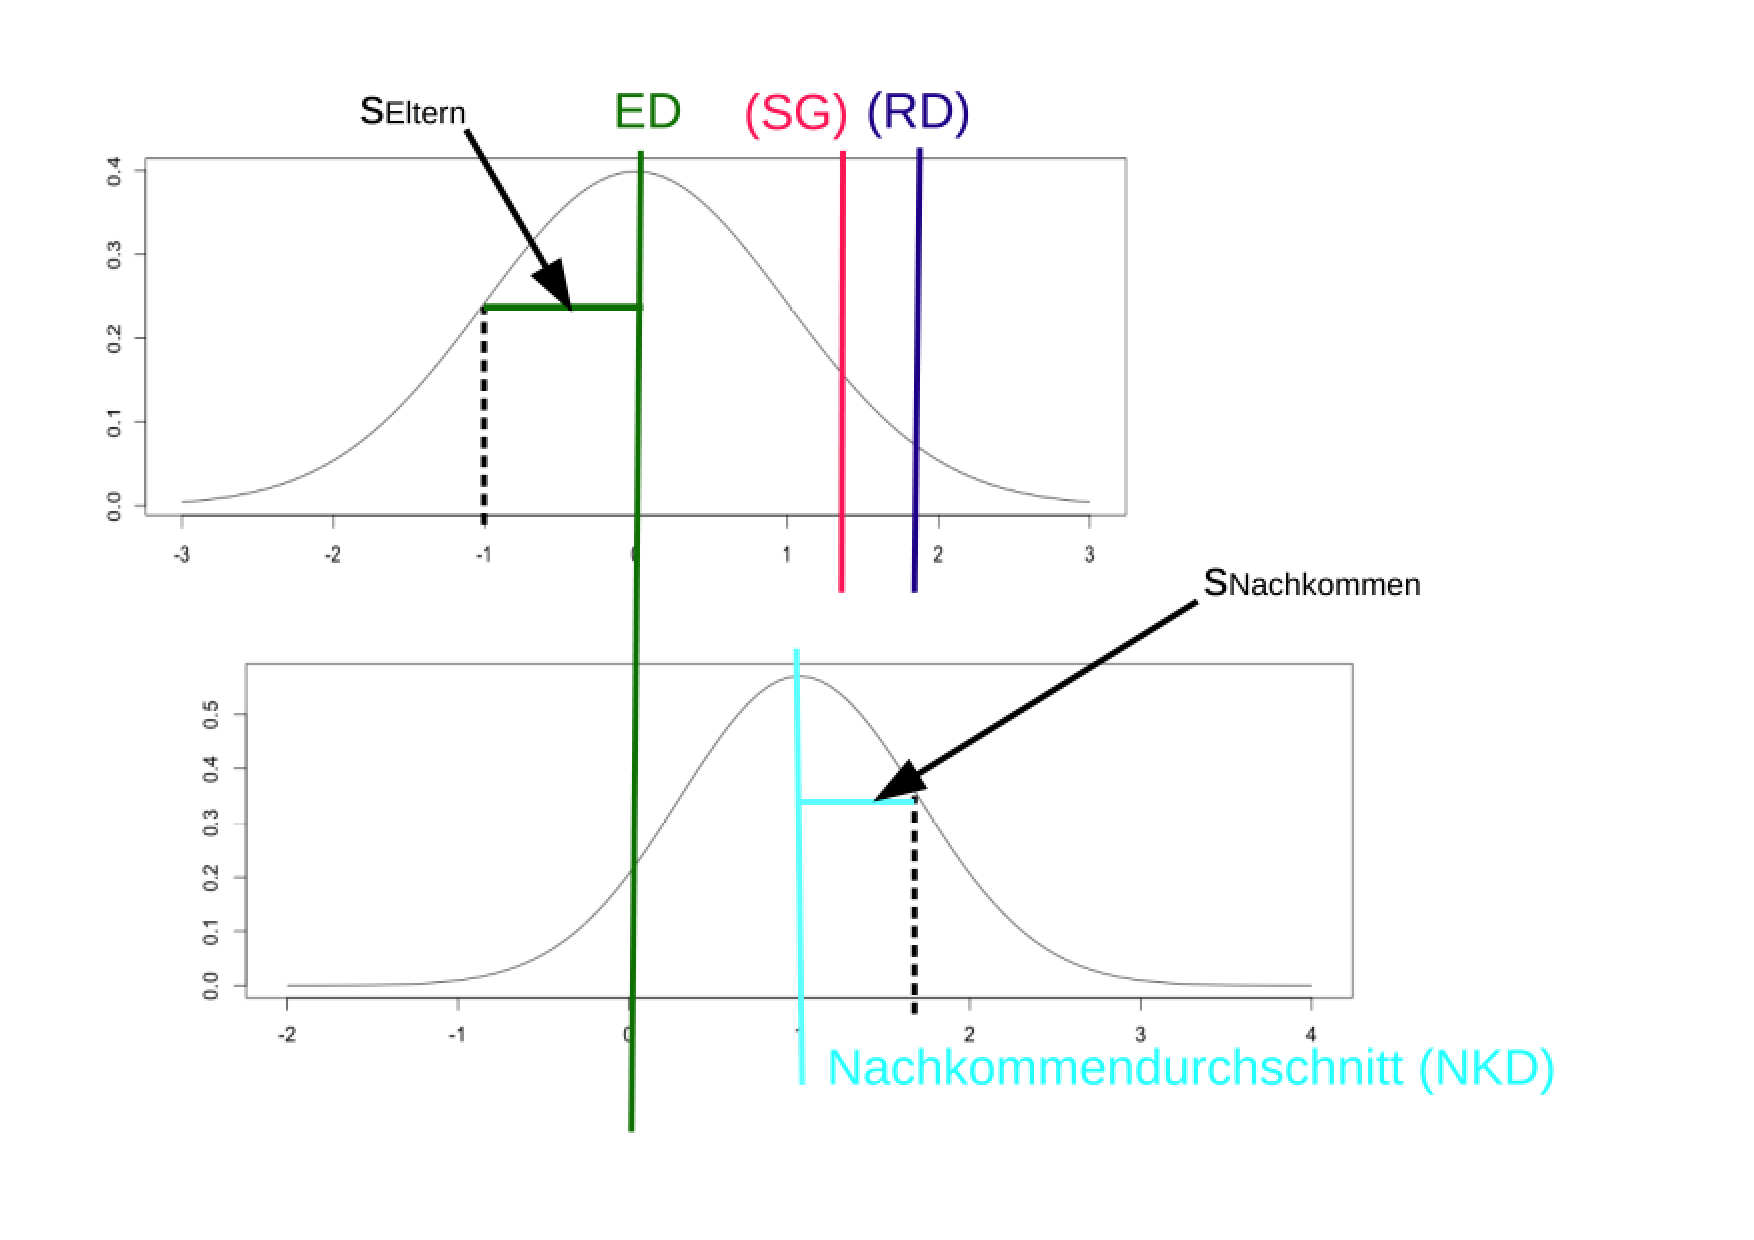
\includegraphics{png/GerichteteSelektionElternNkSol} \end{center}

where

\begin{longtable}[]{@{}ll@{}}
\toprule
Abbreviation & Meaning\tabularnewline
\midrule
\endhead
ED & parent average\tabularnewline
SG & selection threshold\tabularnewline
RD & average of selected parents\tabularnewline
sEltern & standard deviation of parents\tabularnewline
sNachkommen & standard deviation of progeny\tabularnewline
NKD & average of progeny\tabularnewline
\bottomrule
\end{longtable}

\clearpage
\pagebreak

\begin{enumerate}
\item[c)] In pig breeding the two meat quality traits \textbf{tenderness} (ZH) and \textbf{juiciness} (SH) should be considered in the aggregate genotype $H$. The economic values for the two traits are $w_{ZH} = 5$ und $w_{SH} = 1$. Because both traits in the aggregate genotype are difficult to measure, $H$ is estimated using an index $I$ which contains the traits \textbf{sheer force} (SK) and \textbf{drip loss} (SV) beinhaltet. What is the vector $b$ of index weights which follows from selection index theory? 
\end{enumerate}

\subsubsection{Assumptions}\label{assumptions}

\begin{itemize}
\tightlist
\item
  Economic values \(w\) are given as
\end{itemize}

\[w = \left[
\begin{array}{r}
  5 \\ 
  1 \\ 
  \end{array}\right]
\]

\begin{itemize}
\tightlist
\item
  The variance covariance matrix \(P\) between the traits \texttt{SK}
  and \texttt{SV} in the index is
\end{itemize}

\[P = \left[
\begin{array}{rr}
  4 & 0 \\ 
  0 & 10 \\ 
  \end{array}\right]
\]

\begin{itemize}
\tightlist
\item
  The covariance matrix \(G\) between the traits in the index and in the
  aggregate genotype is
\end{itemize}

\[G = \left[
\begin{array}{rr}
  1.0 & -0.2 \\ 
  0.2 & 2.0 \\ 
  \end{array}\right]
\]

\subsubsection{Your Task}\label{your-task-2}

Compute the vector \(b\) of index weights.

\sol

The vector \(b\) is computed base on the following index equations
\[Pb = Gw\]

hence we get \[b = P^{-1}Gw\]

\begin{Shaded}
\begin{Highlighting}[]
\NormalTok{(mat_inv_P <-}\StringTok{ }\KeywordTok{solve}\NormalTok{(matP))}
\end{Highlighting}
\end{Shaded}

\begin{verbatim}
##      [,1] [,2]
## [1,] 0.25  0.0
## [2,] 0.00  0.1
\end{verbatim}

\begin{Shaded}
\begin{Highlighting}[]
\NormalTok{(mat_inv_P }\OperatorTok\StringTok{ }\NormalTok{matG)}
\end{Highlighting}
\end{Shaded}

\begin{verbatim}
##      [,1]  [,2]
## [1,] 0.25 -0.05
## [2,] 0.02  0.20
\end{verbatim}

\[b = \left[
\begin{array}{r}
  1.20 \\ 
  0.30 \\ 
  \end{array}\right]
\]

\clearpage
\pagebreak

\subsection{Problem 4 Inbreeding}\label{problem-4-inbreeding}

\begin{enumerate}
\item[a)] The efficient computation of inbreeding in big pedigrees is baed on the Cholesky-Decomposition of the numerator relationship matrix $A$. Compute the matrix $R$ which results from the Cholesky-Decomposition for the following pedigree.
\points{25}
\end{enumerate}

\begin{verbatim}
##   sire  dam
## 1 <NA> <NA>
## 2 <NA> <NA>
## 3    2    1
## 4    2    1
## 5    3    4
\end{verbatim}

\subsubsection{Hint}\label{hint}

The Cholesky-Decomposition of the matrix \(A\) is \[A = R*R^T\]

\sol

The matrix \(R\) corresponds to

\begin{Shaded}
\begin{Highlighting}[]
\NormalTok{(matR <-}\StringTok{ }\KeywordTok{t}\NormalTok{(}\KeywordTok{chol}\NormalTok{(}\KeywordTok{as.matrix}\NormalTok{(}\KeywordTok{getA}\NormalTok{(ped)))))}
\end{Highlighting}
\end{Shaded}

\begin{verbatim}
##     1   2         3         4         5
## 1 1.0 0.0 0.0000000 0.0000000 0.0000000
## 2 0.0 1.0 0.0000000 0.0000000 0.0000000
## 3 0.5 0.5 0.7071068 0.0000000 0.0000000
## 4 0.5 0.5 0.0000000 0.7071068 0.0000000
## 5 0.5 0.5 0.3535534 0.3535534 0.7071068
\end{verbatim}

\[R = \left[
\begin{array}{rrrrr}
  1.0000 & 0.0000 & 0.0000 & 0.0000 & 0.0000 \\ 
  0.0000 & 1.0000 & 0.0000 & 0.0000 & 0.0000 \\ 
  0.5000 & 0.5000 & 0.7071 & 0.0000 & 0.0000 \\ 
  0.5000 & 0.5000 & 0.0000 & 0.7071 & 0.0000 \\ 
  0.5000 & 0.5000 & 0.3536 & 0.3536 & 0.7071 \\ 
  \end{array}\right]
\]

\clearpage
\pagebreak

\begin{enumerate}
\item[b)] Compute the inbreeding coefficients of the five animals in the pedigree of Problem  4a) based on the values in matrix $R$. 
\points{5}
\end{enumerate}

\sol

The inbreeding coefficients are computed based on the sum of the squared
values of each row of matrix \(R\)

\begin{Shaded}
\begin{Highlighting}[]
\NormalTok{(matR2 <-}\StringTok{ }\NormalTok{matR}\OperatorTok{*}\NormalTok{matR)}
\end{Highlighting}
\end{Shaded}

\begin{verbatim}
##      1    2     3     4   5
## 1 1.00 0.00 0.000 0.000 0.0
## 2 0.00 1.00 0.000 0.000 0.0
## 3 0.25 0.25 0.500 0.000 0.0
## 4 0.25 0.25 0.000 0.500 0.0
## 5 0.25 0.25 0.125 0.125 0.5
\end{verbatim}

\begin{Shaded}
\begin{Highlighting}[]
\NormalTok{(vec_inb <-}\StringTok{ }\KeywordTok{apply}\NormalTok{(matR2, }\DecValTok{1}\NormalTok{, sum) }\OperatorTok{-}\StringTok{ }\DecValTok{1}\NormalTok{)}
\end{Highlighting}
\end{Shaded}

\begin{verbatim}
##    1    2    3    4    5 
## 0.00 0.00 0.00 0.00 0.25
\end{verbatim}

We check with \texttt{pedigreemm()}

\begin{Shaded}
\begin{Highlighting}[]
\KeywordTok{inbreeding}\NormalTok{(}\DataTypeTok{ped =}\NormalTok{ ped)}
\end{Highlighting}
\end{Shaded}

\begin{verbatim}
## [1] 0.00 0.00 0.00 0.00 0.25
\end{verbatim}

\clearpage
\pagebreak

\subsection{Problem 5 Prediction of Breeding
Values}\label{problem-5-prediction-of-breeding-values}

Breeding values should be predicted based on the following data set.

\begin{longtable}[]{@{}llr@{}}
\toprule
Animal & Herd & Observation\tabularnewline
\midrule
\endhead
1 & NA & NA\tabularnewline
2 & NA & NA\tabularnewline
3 & B & 118\tabularnewline
4 & A & 120\tabularnewline
5 & A & 135\tabularnewline
6 & B & 115\tabularnewline
\bottomrule
\end{longtable}

The variances can be taken from the following table.

\begin{longtable}[]{@{}lr@{}}
\toprule
Component & Value\tabularnewline
\midrule
\endhead
phenotypic & 32\tabularnewline
additive genetic & 8\tabularnewline
\bottomrule
\end{longtable}

\begin{enumerate}
\item[a)] Predict the breeding value of the 6 animals based on their own performance where the population mean $\mu$ corresponds to the average of the phenotypic observation 
\points{9}
\end{enumerate}

\sol

The predicted breeding values based on the own performance can be
computed as \[\hat{a}_i = h^2(y_i - \mu)\]

Applying this to the data from the above table, this means

\begin{longtable}[]{@{}lr@{}}
\toprule
Animal & PBV\tabularnewline
\midrule
\endhead
1 & NA\tabularnewline
2 & NA\tabularnewline
3 & -1.00\tabularnewline
4 & -0.50\tabularnewline
5 & 3.25\tabularnewline
6 & -1.75\tabularnewline
\bottomrule
\end{longtable}

\clearpage
\pagebreak

\begin{enumerate}
\item[b)] Predict the breeding values for the animals in the table above using a BLUP animal model. Set up the model and the resulting mixed model equations. Transfer the information from the data into the model by filling the numeric values into the matrices and the vectors where possible. 
\points{16}
\end{enumerate}

\sol

The model corresponds to: \[y = Xb + Za + e\]

\begin{tabular}{lll}
wobei &  &  \\
      & $y$ & vector of all observations \\
      & $b$ & vector of fixed herd effects \\
      & $X$ & incidence matrix linking $b$ and $y$ \\
      & $a$ & vector of random breeding values  \\
      & $Z$ & incidence matrix linking $a$ with $y$ \\
      & $e$ & vector of random residuals
\end{tabular}

Mixed model equations

\subsubsection{\texorpdfstring{Coefficient matrix
\(M\)}{Coefficient matrix M}}\label{coefficient-matrix-m}

To set up the coefficient matrix, we need to know the incidence matrices
\(X\) and \(Z\).

\begin{Shaded}
\begin{Highlighting}[]
\NormalTok{(X <-}\StringTok{ }\KeywordTok{matrix}\NormalTok{(}\DataTypeTok{data =} \KeywordTok{c}\NormalTok{(}\DecValTok{0}\NormalTok{, }\DecValTok{1}\NormalTok{,}
                     \DecValTok{1}\NormalTok{, }\DecValTok{0}\NormalTok{,}
                     \DecValTok{1}\NormalTok{, }\DecValTok{0}\NormalTok{,}
                     \DecValTok{0}\NormalTok{, }\DecValTok{1}\NormalTok{), }\DataTypeTok{ncol =} \DecValTok{2}\NormalTok{, }\DataTypeTok{byrow =} \OtherTok{TRUE}\NormalTok{))}
\end{Highlighting}
\end{Shaded}

\begin{verbatim}
##      [,1] [,2]
## [1,]    0    1
## [2,]    1    0
## [3,]    1    0
## [4,]    0    1
\end{verbatim}

\begin{Shaded}
\begin{Highlighting}[]
\NormalTok{(Z <-}\StringTok{ }\KeywordTok{cbind}\NormalTok{(}\KeywordTok{matrix}\NormalTok{(}\DataTypeTok{data =} \DecValTok{0}\NormalTok{, }\DataTypeTok{nrow =} \DecValTok{4}\NormalTok{, }\DataTypeTok{ncol =} \DecValTok{2}\NormalTok{), }\KeywordTok{diag}\NormalTok{(}\DecValTok{4}\NormalTok{)))}
\end{Highlighting}
\end{Shaded}

\begin{verbatim}
##      [,1] [,2] [,3] [,4] [,5] [,6]
## [1,]    0    0    1    0    0    0
## [2,]    0    0    0    1    0    0
## [3,]    0    0    0    0    1    0
## [4,]    0    0    0    0    0    1
\end{verbatim}

The four sub-matrices of \(M\) are

\begin{enumerate}
\def\labelenumi{\arabic{enumi}.}
\tightlist
\item
  \(X^TX\)
\end{enumerate}

\begin{Shaded}
\begin{Highlighting}[]
\NormalTok{(XTX <-}\StringTok{ }\KeywordTok{t}\NormalTok{(X) }\OperatorTok\StringTok{ }\NormalTok{X)}
\end{Highlighting}
\end{Shaded}

\begin{verbatim}
##      [,1] [,2]
## [1,]    2    0
## [2,]    0    2
\end{verbatim}

\begin{enumerate}
\def\labelenumi{\arabic{enumi}.}
\setcounter{enumi}{1}
\tightlist
\item
  \(X^TZ\)
\end{enumerate}

\begin{Shaded}
\begin{Highlighting}[]
\NormalTok{(XTZ <-}\StringTok{ }\KeywordTok{t}\NormalTok{(X) }\OperatorTok\StringTok{ }\NormalTok{Z)}
\end{Highlighting}
\end{Shaded}

\begin{verbatim}
##      [,1] [,2] [,3] [,4] [,5] [,6]
## [1,]    0    0    0    1    1    0
## [2,]    0    0    1    0    0    1
\end{verbatim}

\begin{enumerate}
\def\labelenumi{\arabic{enumi}.}
\setcounter{enumi}{2}
\tightlist
\item
  \(Z^TX\)
\end{enumerate}

\begin{Shaded}
\begin{Highlighting}[]
\NormalTok{(ZTX <-}\StringTok{ }\KeywordTok{t}\NormalTok{(XTZ))}
\end{Highlighting}
\end{Shaded}

\begin{verbatim}
##      [,1] [,2]
## [1,]    0    0
## [2,]    0    0
## [3,]    0    1
## [4,]    1    0
## [5,]    1    0
## [6,]    0    1
\end{verbatim}

\begin{enumerate}
\def\labelenumi{\arabic{enumi}.}
\setcounter{enumi}{3}
\tightlist
\item
  \(Z^TZ + A^{-1}\alpha\)
\end{enumerate}

\begin{Shaded}
\begin{Highlighting}[]
\NormalTok{Ainv <-}\StringTok{ }\KeywordTok{diag}\NormalTok{(nNrRecords)}
\NormalTok{(ZTZAinvAlpha <-}\StringTok{ }\KeywordTok{t}\NormalTok{(Z) }\OperatorTok\StringTok{ }\NormalTok{Z }\OperatorTok{+}\StringTok{ }\NormalTok{Ainv }\OperatorTok{*}\StringTok{ }\NormalTok{alpha)}
\end{Highlighting}
\end{Shaded}

\begin{verbatim}
##      [,1] [,2] [,3] [,4] [,5] [,6]
## [1,]    3    0    0    0    0    0
## [2,]    0    3    0    0    0    0
## [3,]    0    0    4    0    0    0
## [4,]    0    0    0    4    0    0
## [5,]    0    0    0    0    4    0
## [6,]    0    0    0    0    0    4
\end{verbatim}

Setting up of \(M\)

\begin{Shaded}
\begin{Highlighting}[]
\NormalTok{(M <-}\StringTok{ }\KeywordTok{rbind}\NormalTok{(}\KeywordTok{cbind}\NormalTok{(XTX, XTZ), }\KeywordTok{cbind}\NormalTok{(ZTX, ZTZAinvAlpha)))}
\end{Highlighting}
\end{Shaded}

\begin{verbatim}
##      [,1] [,2] [,3] [,4] [,5] [,6] [,7] [,8]
## [1,]    2    0    0    0    0    1    1    0
## [2,]    0    2    0    0    1    0    0    1
## [3,]    0    0    3    0    0    0    0    0
## [4,]    0    0    0    3    0    0    0    0
## [5,]    0    1    0    0    4    0    0    0
## [6,]    1    0    0    0    0    4    0    0
## [7,]    1    0    0    0    0    0    4    0
## [8,]    0    1    0    0    0    0    0    4
\end{verbatim}

\subsubsection{The right-hand side (rhs)}\label{the-right-hand-side-rhs}

The vector \(y\) is obtained from the data

\begin{Shaded}
\begin{Highlighting}[]
\NormalTok{(y <-}\StringTok{ }\NormalTok{dfMlrData}\OperatorTok{$}\NormalTok{Observation[}\OperatorTok{!}\KeywordTok{is.na}\NormalTok{(dfMlrData}\OperatorTok{$}\NormalTok{Observation)])}
\end{Highlighting}
\end{Shaded}

\begin{verbatim}
## [1] 118 120 135 115
\end{verbatim}

\begin{enumerate}
\def\labelenumi{\arabic{enumi}.}
\tightlist
\item
  \(X^Ty\)
\end{enumerate}

\begin{Shaded}
\begin{Highlighting}[]
\NormalTok{(XTy <-}\StringTok{ }\KeywordTok{t}\NormalTok{(X) }\OperatorTok\StringTok{ }\NormalTok{y)}
\end{Highlighting}
\end{Shaded}

\begin{verbatim}
##      [,1]
## [1,]  255
## [2,]  233
\end{verbatim}

\begin{enumerate}
\def\labelenumi{\arabic{enumi}.}
\setcounter{enumi}{1}
\tightlist
\item
  \(Z^Ty\)
\end{enumerate}

\begin{Shaded}
\begin{Highlighting}[]
\NormalTok{(ZTy <-}\StringTok{ }\KeywordTok{t}\NormalTok{(Z) }\OperatorTok\StringTok{ }\NormalTok{y)}
\end{Highlighting}
\end{Shaded}

\begin{verbatim}
##      [,1]
## [1,]    0
## [2,]    0
## [3,]  118
## [4,]  120
## [5,]  135
## [6,]  115
\end{verbatim}

Setting up rhs

\begin{Shaded}
\begin{Highlighting}[]
\NormalTok{(rhs <-}\StringTok{  }\KeywordTok{rbind}\NormalTok{(XTy,ZTy))}
\end{Highlighting}
\end{Shaded}

\begin{verbatim}
##      [,1]
## [1,]  255
## [2,]  233
## [3,]    0
## [4,]    0
## [5,]  118
## [6,]  120
## [7,]  135
## [8,]  115
\end{verbatim}

\subsubsection{Solution}\label{solution}

The solution is obtained as \(sol = M^{-1} * rhs\)

\begin{Shaded}
\begin{Highlighting}[]
\NormalTok{(sol <-}\StringTok{ }\KeywordTok{solve}\NormalTok{(M, rhs))}
\end{Highlighting}
\end{Shaded}

\begin{verbatim}
##         [,1]
## [1,] 127.500
## [2,] 116.500
## [3,]   0.000
## [4,]   0.000
## [5,]   0.375
## [6,]  -1.875
## [7,]   1.875
## [8,]  -0.375
\end{verbatim}

\clearpage
\pagebreak

\begin{enumerate}
\item[c)] What are the differences when comparing the result from Problem a) and b)?
\points{4}
\end{enumerate}

\sol

\begin{itemize}
\tightlist
\item
  In a) only animals with an own performance get a predicted breeding
  value. In b) all animals get a predicted breeding value.
\item
  In a) the population mean is used to account for environmental
  effects, in b) also herd effects are accounted for.
\end{itemize}


\end{document}
